% Options for packages loaded elsewhere
\PassOptionsToPackage{unicode}{hyperref}
\PassOptionsToPackage{hyphens}{url}
%
\documentclass[
]{article}
\usepackage{lmodern}
\usepackage{amssymb,amsmath}
\usepackage{ifxetex,ifluatex}
\ifnum 0\ifxetex 1\fi\ifluatex 1\fi=0 % if pdftex
  \usepackage[T1]{fontenc}
  \usepackage[utf8]{inputenc}
  \usepackage{textcomp} % provide euro and other symbols
\else % if luatex or xetex
  \usepackage{unicode-math}
  \defaultfontfeatures{Scale=MatchLowercase}
  \defaultfontfeatures[\rmfamily]{Ligatures=TeX,Scale=1}
\fi
% Use upquote if available, for straight quotes in verbatim environments
\IfFileExists{upquote.sty}{\usepackage{upquote}}{}
\IfFileExists{microtype.sty}{% use microtype if available
  \usepackage[]{microtype}
  \UseMicrotypeSet[protrusion]{basicmath} % disable protrusion for tt fonts
}{}
\makeatletter
\@ifundefined{KOMAClassName}{% if non-KOMA class
  \IfFileExists{parskip.sty}{%
    \usepackage{parskip}
  }{% else
    \setlength{\parindent}{0pt}
    \setlength{\parskip}{6pt plus 2pt minus 1pt}}
}{% if KOMA class
  \KOMAoptions{parskip=half}}
\makeatother
\usepackage{xcolor}
\IfFileExists{xurl.sty}{\usepackage{xurl}}{} % add URL line breaks if available
\IfFileExists{bookmark.sty}{\usepackage{bookmark}}{\usepackage{hyperref}}
\hypersetup{
  pdftitle={Untitled},
  pdfauthor={Jared Flater},
  hidelinks,
  pdfcreator={LaTeX via pandoc}}
\urlstyle{same} % disable monospaced font for URLs
\usepackage[margin=1in]{geometry}
\usepackage{color}
\usepackage{fancyvrb}
\newcommand{\VerbBar}{|}
\newcommand{\VERB}{\Verb[commandchars=\\\{\}]}
\DefineVerbatimEnvironment{Highlighting}{Verbatim}{commandchars=\\\{\}}
% Add ',fontsize=\small' for more characters per line
\usepackage{framed}
\definecolor{shadecolor}{RGB}{248,248,248}
\newenvironment{Shaded}{\begin{snugshade}}{\end{snugshade}}
\newcommand{\AlertTok}[1]{\textcolor[rgb]{0.94,0.16,0.16}{#1}}
\newcommand{\AnnotationTok}[1]{\textcolor[rgb]{0.56,0.35,0.01}{\textbf{\textit{#1}}}}
\newcommand{\AttributeTok}[1]{\textcolor[rgb]{0.77,0.63,0.00}{#1}}
\newcommand{\BaseNTok}[1]{\textcolor[rgb]{0.00,0.00,0.81}{#1}}
\newcommand{\BuiltInTok}[1]{#1}
\newcommand{\CharTok}[1]{\textcolor[rgb]{0.31,0.60,0.02}{#1}}
\newcommand{\CommentTok}[1]{\textcolor[rgb]{0.56,0.35,0.01}{\textit{#1}}}
\newcommand{\CommentVarTok}[1]{\textcolor[rgb]{0.56,0.35,0.01}{\textbf{\textit{#1}}}}
\newcommand{\ConstantTok}[1]{\textcolor[rgb]{0.00,0.00,0.00}{#1}}
\newcommand{\ControlFlowTok}[1]{\textcolor[rgb]{0.13,0.29,0.53}{\textbf{#1}}}
\newcommand{\DataTypeTok}[1]{\textcolor[rgb]{0.13,0.29,0.53}{#1}}
\newcommand{\DecValTok}[1]{\textcolor[rgb]{0.00,0.00,0.81}{#1}}
\newcommand{\DocumentationTok}[1]{\textcolor[rgb]{0.56,0.35,0.01}{\textbf{\textit{#1}}}}
\newcommand{\ErrorTok}[1]{\textcolor[rgb]{0.64,0.00,0.00}{\textbf{#1}}}
\newcommand{\ExtensionTok}[1]{#1}
\newcommand{\FloatTok}[1]{\textcolor[rgb]{0.00,0.00,0.81}{#1}}
\newcommand{\FunctionTok}[1]{\textcolor[rgb]{0.00,0.00,0.00}{#1}}
\newcommand{\ImportTok}[1]{#1}
\newcommand{\InformationTok}[1]{\textcolor[rgb]{0.56,0.35,0.01}{\textbf{\textit{#1}}}}
\newcommand{\KeywordTok}[1]{\textcolor[rgb]{0.13,0.29,0.53}{\textbf{#1}}}
\newcommand{\NormalTok}[1]{#1}
\newcommand{\OperatorTok}[1]{\textcolor[rgb]{0.81,0.36,0.00}{\textbf{#1}}}
\newcommand{\OtherTok}[1]{\textcolor[rgb]{0.56,0.35,0.01}{#1}}
\newcommand{\PreprocessorTok}[1]{\textcolor[rgb]{0.56,0.35,0.01}{\textit{#1}}}
\newcommand{\RegionMarkerTok}[1]{#1}
\newcommand{\SpecialCharTok}[1]{\textcolor[rgb]{0.00,0.00,0.00}{#1}}
\newcommand{\SpecialStringTok}[1]{\textcolor[rgb]{0.31,0.60,0.02}{#1}}
\newcommand{\StringTok}[1]{\textcolor[rgb]{0.31,0.60,0.02}{#1}}
\newcommand{\VariableTok}[1]{\textcolor[rgb]{0.00,0.00,0.00}{#1}}
\newcommand{\VerbatimStringTok}[1]{\textcolor[rgb]{0.31,0.60,0.02}{#1}}
\newcommand{\WarningTok}[1]{\textcolor[rgb]{0.56,0.35,0.01}{\textbf{\textit{#1}}}}
\usepackage{graphicx,grffile}
\makeatletter
\def\maxwidth{\ifdim\Gin@nat@width>\linewidth\linewidth\else\Gin@nat@width\fi}
\def\maxheight{\ifdim\Gin@nat@height>\textheight\textheight\else\Gin@nat@height\fi}
\makeatother
% Scale images if necessary, so that they will not overflow the page
% margins by default, and it is still possible to overwrite the defaults
% using explicit options in \includegraphics[width, height, ...]{}
\setkeys{Gin}{width=\maxwidth,height=\maxheight,keepaspectratio}
% Set default figure placement to htbp
\makeatletter
\def\fps@figure{htbp}
\makeatother
\setlength{\emergencystretch}{3em} % prevent overfull lines
\providecommand{\tightlist}{%
  \setlength{\itemsep}{0pt}\setlength{\parskip}{0pt}}
\setcounter{secnumdepth}{-\maxdimen} % remove section numbering

\title{Untitled}
\author{Jared Flater}
\date{10/8/2020}

\begin{document}
\maketitle

\begin{Shaded}
\begin{Highlighting}[]
\KeywordTok{library}\NormalTok{(tidyverse)}
\end{Highlighting}
\end{Shaded}

\begin{verbatim}
## -- Attaching packages --------------------------------------------------------------------------------------------------------- tidyverse 1.3.0 --
\end{verbatim}

\begin{verbatim}
## v ggplot2 3.3.2     v purrr   0.3.4
## v tibble  3.0.3     v dplyr   1.0.2
## v tidyr   1.1.2     v stringr 1.4.0
## v readr   1.4.0     v forcats 0.5.0
\end{verbatim}

\begin{verbatim}
## -- Conflicts ------------------------------------------------------------------------------------------------------------ tidyverse_conflicts() --
## x dplyr::filter() masks stats::filter()
## x dplyr::lag()    masks stats::lag()
\end{verbatim}

\begin{Shaded}
\begin{Highlighting}[]
\KeywordTok{library}\NormalTok{(phyloseq)}
\KeywordTok{library}\NormalTok{(phylosmith)}
\end{Highlighting}
\end{Shaded}

\hypertarget{worle-soil}{%
\section{Worle soil}\label{worle-soil}}

This data now includes bacterial communities from soil samples from the
WOR rainfall experiment.

\begin{Shaded}
\begin{Highlighting}[]
\NormalTok{soil <-}\StringTok{ }\KeywordTok{subset_samples}\NormalTok{(worle, matrix }\OperatorTok{==}\StringTok{ }\KeywordTok{c}\NormalTok{(}\StringTok{"soil"}\NormalTok{))}
\KeywordTok{head}\NormalTok{(}\KeywordTok{sample_data}\NormalTok{(soil))}
\end{Highlighting}
\end{Shaded}

\begin{verbatim}
##                 unique_id     experiment matrix       treatment plot sample_day
## P1-s1-d1-b     P1-s1-d1-b Worle_Rainfall   soil no_manure_strip    1   Baseline
## P1-s1-d1-t0   P1-s1-d1-t0 Worle_Rainfall   soil no_manure_strip    1       T000
## P1-s1-d1-t14 P1-s1-d1-t14 Worle_Rainfall   soil no_manure_strip    1       T014
## P1-s1-d1-t2   P1-s1-d1-t2 Worle_Rainfall   soil no_manure_strip    1       T002
## P1-s1-d2-t2   P1-s1-d2-t2 Worle_Rainfall   soil no_manure_strip    1       T002
## P1-s1-d1-t21 P1-s1-d1-t21 Worle_Rainfall   soil no_manure_strip    1       T021
##              depth in_plot_location block strip manure_treatment soil_type
## P1-s1-d1-b       1               s1     1     Y                N      crop
## P1-s1-d1-t0      1               s1     1     Y                N      crop
## P1-s1-d1-t14     1               s1     1     Y                N      crop
## P1-s1-d1-t2      1               s1     1     Y                N      crop
## P1-s1-d2-t2      2               s1     1     Y                N      crop
## P1-s1-d1-t21     1               s1     1     Y                N      crop
\end{verbatim}

\hypertarget{are-bacterial-communities-in-soil-from-strip-different-from-crop}{%
\section{Are bacterial communities in soil from strip different from
crop?}\label{are-bacterial-communities-in-soil-from-strip-different-from-crop}}

Look at all baseline samples, before manure was applied. Depth is a
strong driver of clustering. Seperate into two datasets by depth, S1 and
S2.

\begin{Shaded}
\begin{Highlighting}[]
\NormalTok{s1 <-}\StringTok{ }\KeywordTok{subset_samples}\NormalTok{(soil, depth }\OperatorTok{==}\StringTok{ }\DecValTok{1}\NormalTok{)}
\NormalTok{s2 <-}\StringTok{ }\KeywordTok{subset_samples}\NormalTok{(soil, depth }\OperatorTok{==}\StringTok{ }\DecValTok{2}\NormalTok{)}
\end{Highlighting}
\end{Shaded}

Visualize if samples from crop are different from prairie. Select
baseline samples and plot PCoA ordinations.

\begin{Shaded}
\begin{Highlighting}[]
\NormalTok{s1plot <-}\StringTok{ }\NormalTok{s1 }\OperatorTok
\StringTok{  }\KeywordTok{subset_samples}\NormalTok{(sample_day }\OperatorTok{==}\StringTok{ }\KeywordTok{c}\NormalTok{(}\StringTok{"Baseline"}\NormalTok{)) }\OperatorTok
\StringTok{  }\KeywordTok{pcoa_phyloseq}\NormalTok{(}\KeywordTok{c}\NormalTok{(}\StringTok{'soil_type'}\NormalTok{), }\DataTypeTok{circle =} \OtherTok{TRUE}\NormalTok{)}
\NormalTok{s2plot <-}\StringTok{ }\NormalTok{s2 }\OperatorTok
\StringTok{  }\KeywordTok{subset_samples}\NormalTok{(sample_day }\OperatorTok{==}\StringTok{ }\KeywordTok{c}\NormalTok{(}\StringTok{"Baseline"}\NormalTok{)) }\OperatorTok
\StringTok{  }\KeywordTok{pcoa_phyloseq}\NormalTok{(}\KeywordTok{c}\NormalTok{(}\StringTok{'soil_type'}\NormalTok{), }\DataTypeTok{circle =} \OtherTok{TRUE}\NormalTok{)}
\NormalTok{s1plot}
\end{Highlighting}
\end{Shaded}

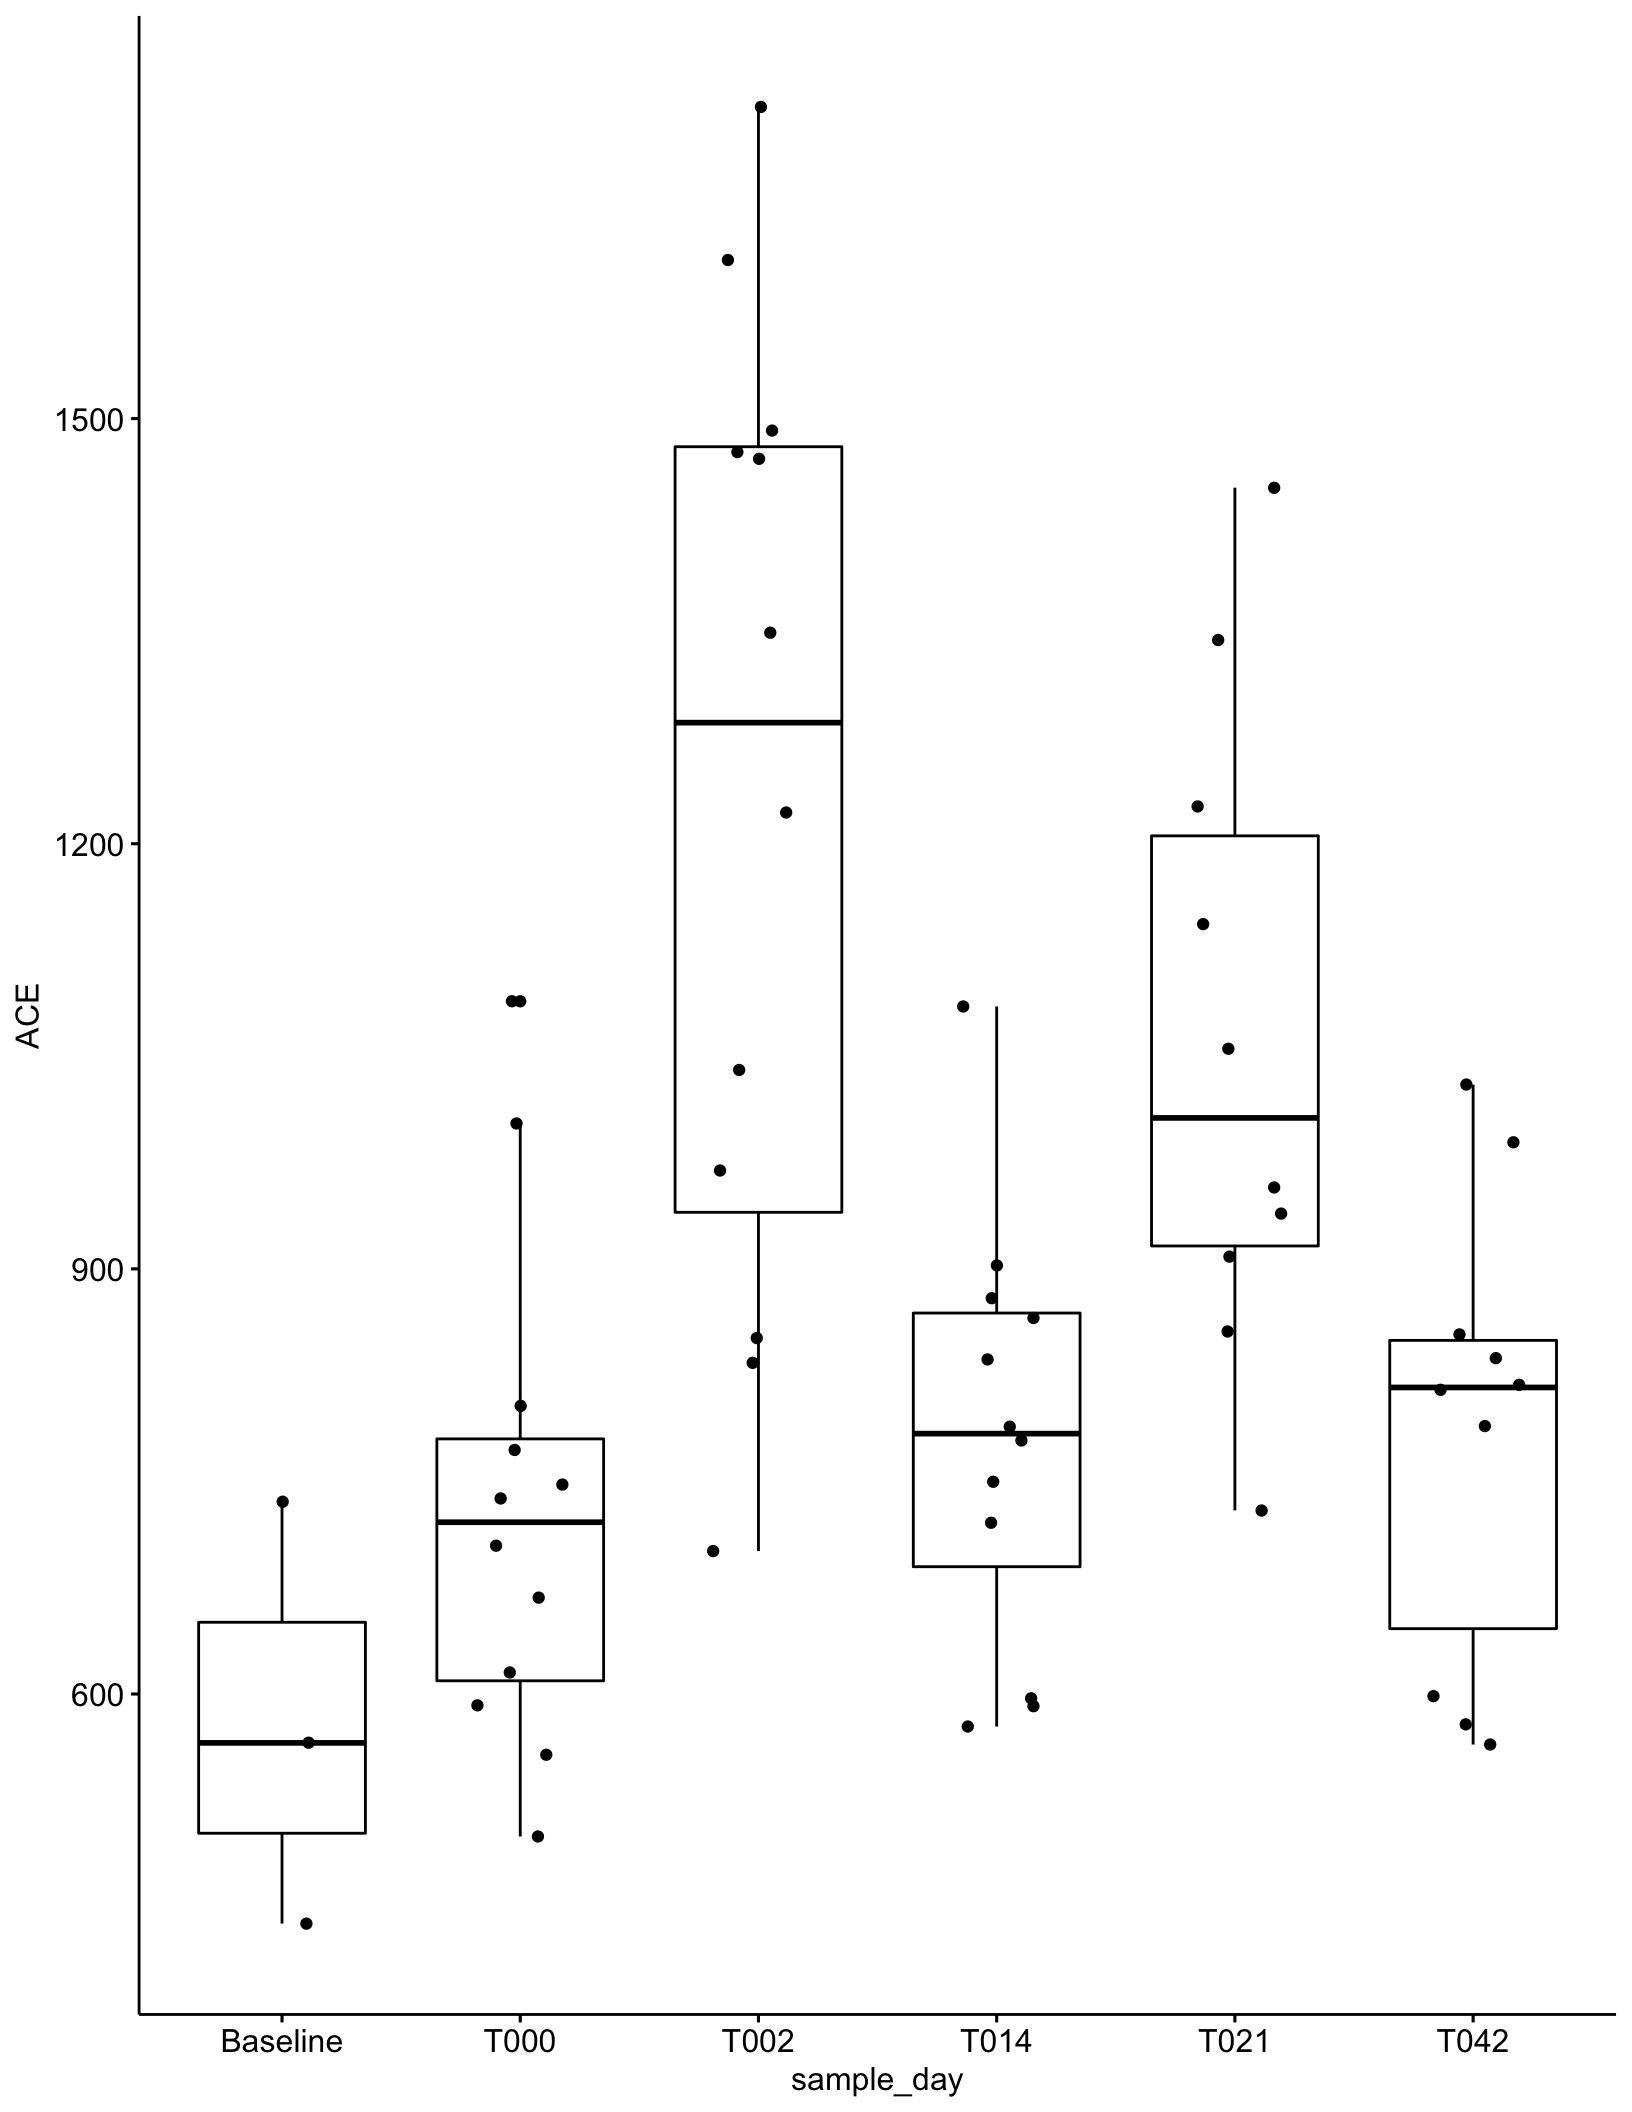
\includegraphics{cropprairiebetadiversity_files/figure-latex/unnamed-chunk-4-1.pdf}

\begin{Shaded}
\begin{Highlighting}[]
\NormalTok{s2plot}
\end{Highlighting}
\end{Shaded}

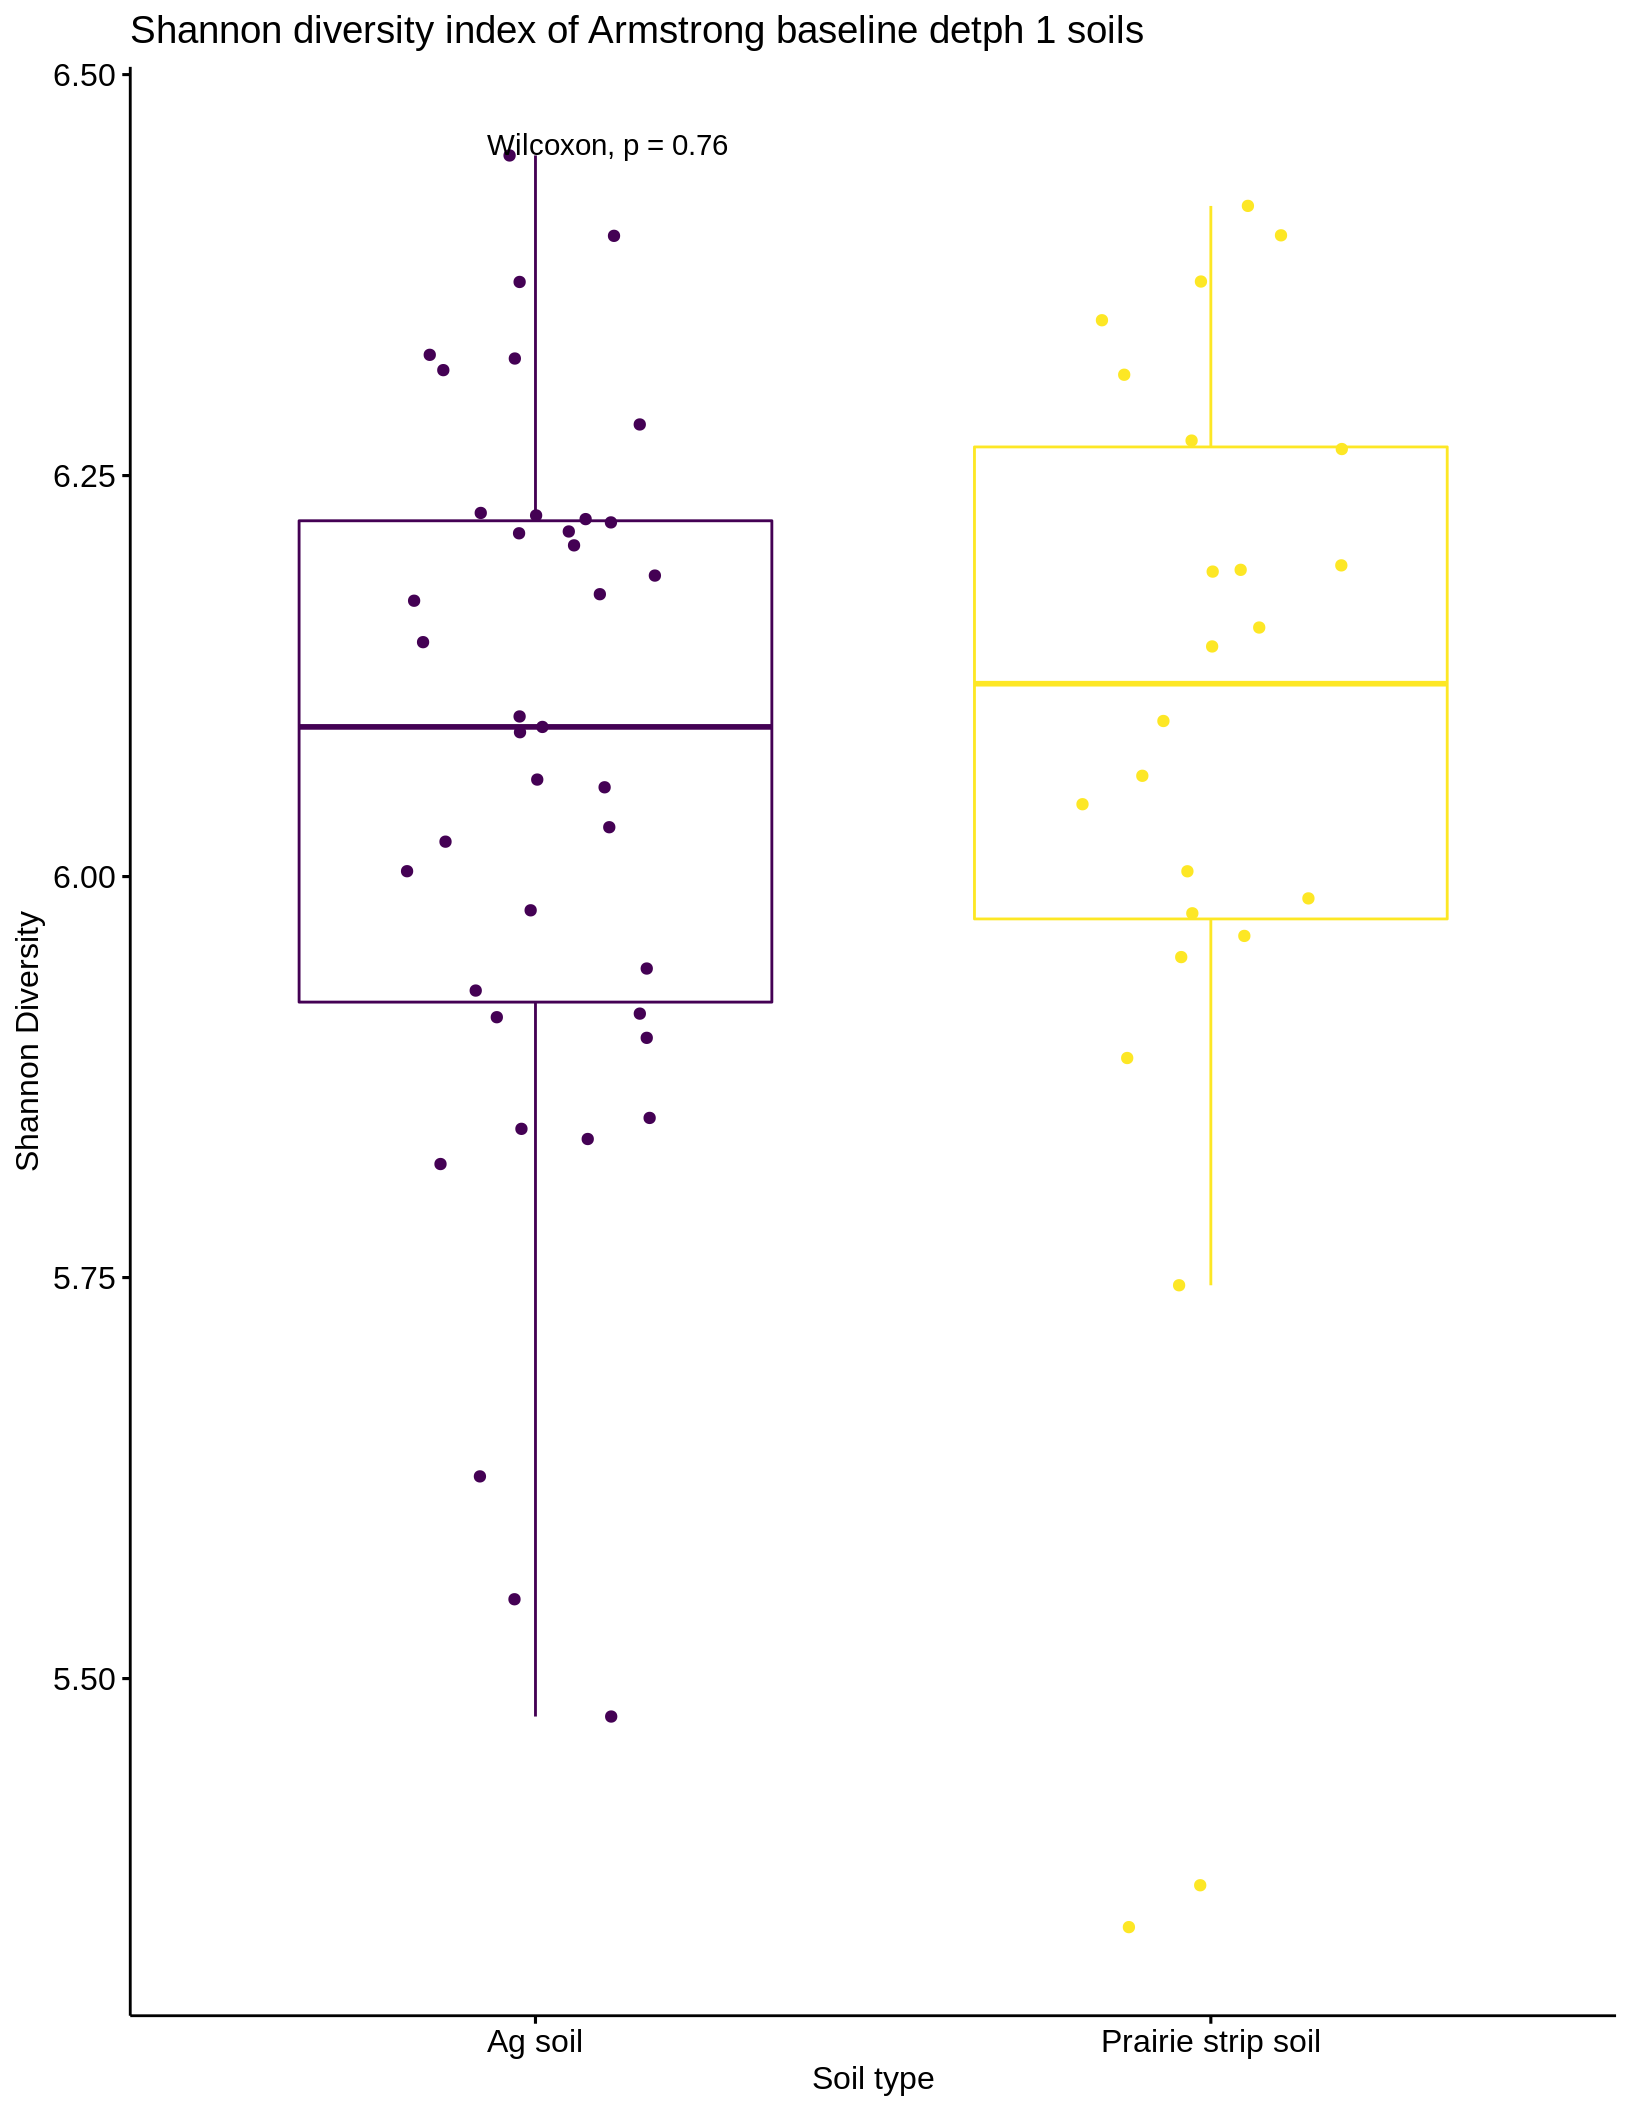
\includegraphics{cropprairiebetadiversity_files/figure-latex/unnamed-chunk-4-2.pdf}
Rarefied and mintax 10

\begin{Shaded}
\begin{Highlighting}[]
\NormalTok{d1rmintax10 <-}\StringTok{ }\KeywordTok{subset_samples}\NormalTok{(soil, depth }\OperatorTok{==}\StringTok{ }\DecValTok{1} \OperatorTok{&}\StringTok{ }\NormalTok{sample_day }\OperatorTok{==}\StringTok{ }\KeywordTok{c}\NormalTok{(}\StringTok{"Baseline"}\NormalTok{)) }\OperatorTok
\StringTok{  }\KeywordTok{rarefy_even_depth}\NormalTok{(}\DataTypeTok{sample.size =} \DecValTok{10000}\NormalTok{, }\DataTypeTok{rngseed =} \DecValTok{1231}\NormalTok{, }\DataTypeTok{replace =}\NormalTok{ T) }\OperatorTok
\StringTok{  }\KeywordTok{filter_taxa}\NormalTok{(}\ControlFlowTok{function}\NormalTok{(x) }\KeywordTok{sum}\NormalTok{(x) }\OperatorTok{>=}\StringTok{ }\DecValTok{10}\NormalTok{, T) }\OperatorTok
\StringTok{  }\KeywordTok{pcoa_phyloseq}\NormalTok{(}\KeywordTok{c}\NormalTok{(}\StringTok{'soil_type'}\NormalTok{), }\DataTypeTok{circle =} \OtherTok{TRUE}\NormalTok{)}
\end{Highlighting}
\end{Shaded}

\begin{verbatim}
## `set.seed(1231)` was used to initialize repeatable random subsampling.
\end{verbatim}

\begin{verbatim}
## Please record this for your records so others can reproduce.
\end{verbatim}

\begin{verbatim}
## Try `set.seed(1231); .Random.seed` for the full vector
\end{verbatim}

\begin{verbatim}
## ...
\end{verbatim}

\begin{verbatim}
## 32 samples removedbecause they contained fewer reads than `sample.size`.
\end{verbatim}

\begin{verbatim}
## Up to first five removed samples are:
\end{verbatim}

\begin{verbatim}
## P1-s3-d1-bP1-s6-d1-bP1-s9-d1-bP2-s2-d1-bP2-s6-d1-b
\end{verbatim}

\begin{verbatim}
## ...
\end{verbatim}

\begin{verbatim}
## 74006OTUs were removed because they are no longer 
## present in any sample after random subsampling
\end{verbatim}

\begin{verbatim}
## ...
\end{verbatim}

\begin{Shaded}
\begin{Highlighting}[]
\NormalTok{d2rmintax10 <-}\StringTok{ }\KeywordTok{subset_samples}\NormalTok{(soil, depth }\OperatorTok{==}\StringTok{ }\DecValTok{2} \OperatorTok{&}\StringTok{ }\NormalTok{sample_day }\OperatorTok{==}\StringTok{ }\KeywordTok{c}\NormalTok{(}\StringTok{"Baseline"}\NormalTok{)) }\OperatorTok
\StringTok{  }\KeywordTok{rarefy_even_depth}\NormalTok{(}\DataTypeTok{sample.size =} \DecValTok{10000}\NormalTok{, }\DataTypeTok{rngseed =} \DecValTok{1231}\NormalTok{, }\DataTypeTok{replace =}\NormalTok{ T) }\OperatorTok
\StringTok{  }\KeywordTok{filter_taxa}\NormalTok{(}\ControlFlowTok{function}\NormalTok{(x) }\KeywordTok{sum}\NormalTok{(x) }\OperatorTok{>=}\StringTok{ }\DecValTok{10}\NormalTok{, T) }\OperatorTok
\StringTok{  }\KeywordTok{pcoa_phyloseq}\NormalTok{(}\KeywordTok{c}\NormalTok{(}\StringTok{'soil_type'}\NormalTok{), }\DataTypeTok{circle =} \OtherTok{TRUE}\NormalTok{)}
\end{Highlighting}
\end{Shaded}

\begin{verbatim}
## `set.seed(1231)` was used to initialize repeatable random subsampling.
\end{verbatim}

\begin{verbatim}
## Please record this for your records so others can reproduce.
\end{verbatim}

\begin{verbatim}
## Try `set.seed(1231); .Random.seed` for the full vector
\end{verbatim}

\begin{verbatim}
## ...
\end{verbatim}

\begin{verbatim}
## 13 samples removedbecause they contained fewer reads than `sample.size`.
\end{verbatim}

\begin{verbatim}
## Up to first five removed samples are:
\end{verbatim}

\begin{verbatim}
## P1-s4-d2-bP1-s5-d2-bP1-s6-d2-bP2-s3-d2-bP2-s4-d2-b
\end{verbatim}

\begin{verbatim}
## ...
\end{verbatim}

\begin{verbatim}
## 69113OTUs were removed because they are no longer 
## present in any sample after random subsampling
\end{verbatim}

\begin{verbatim}
## ...
\end{verbatim}

\begin{Shaded}
\begin{Highlighting}[]
\NormalTok{d1rmintax10}
\end{Highlighting}
\end{Shaded}

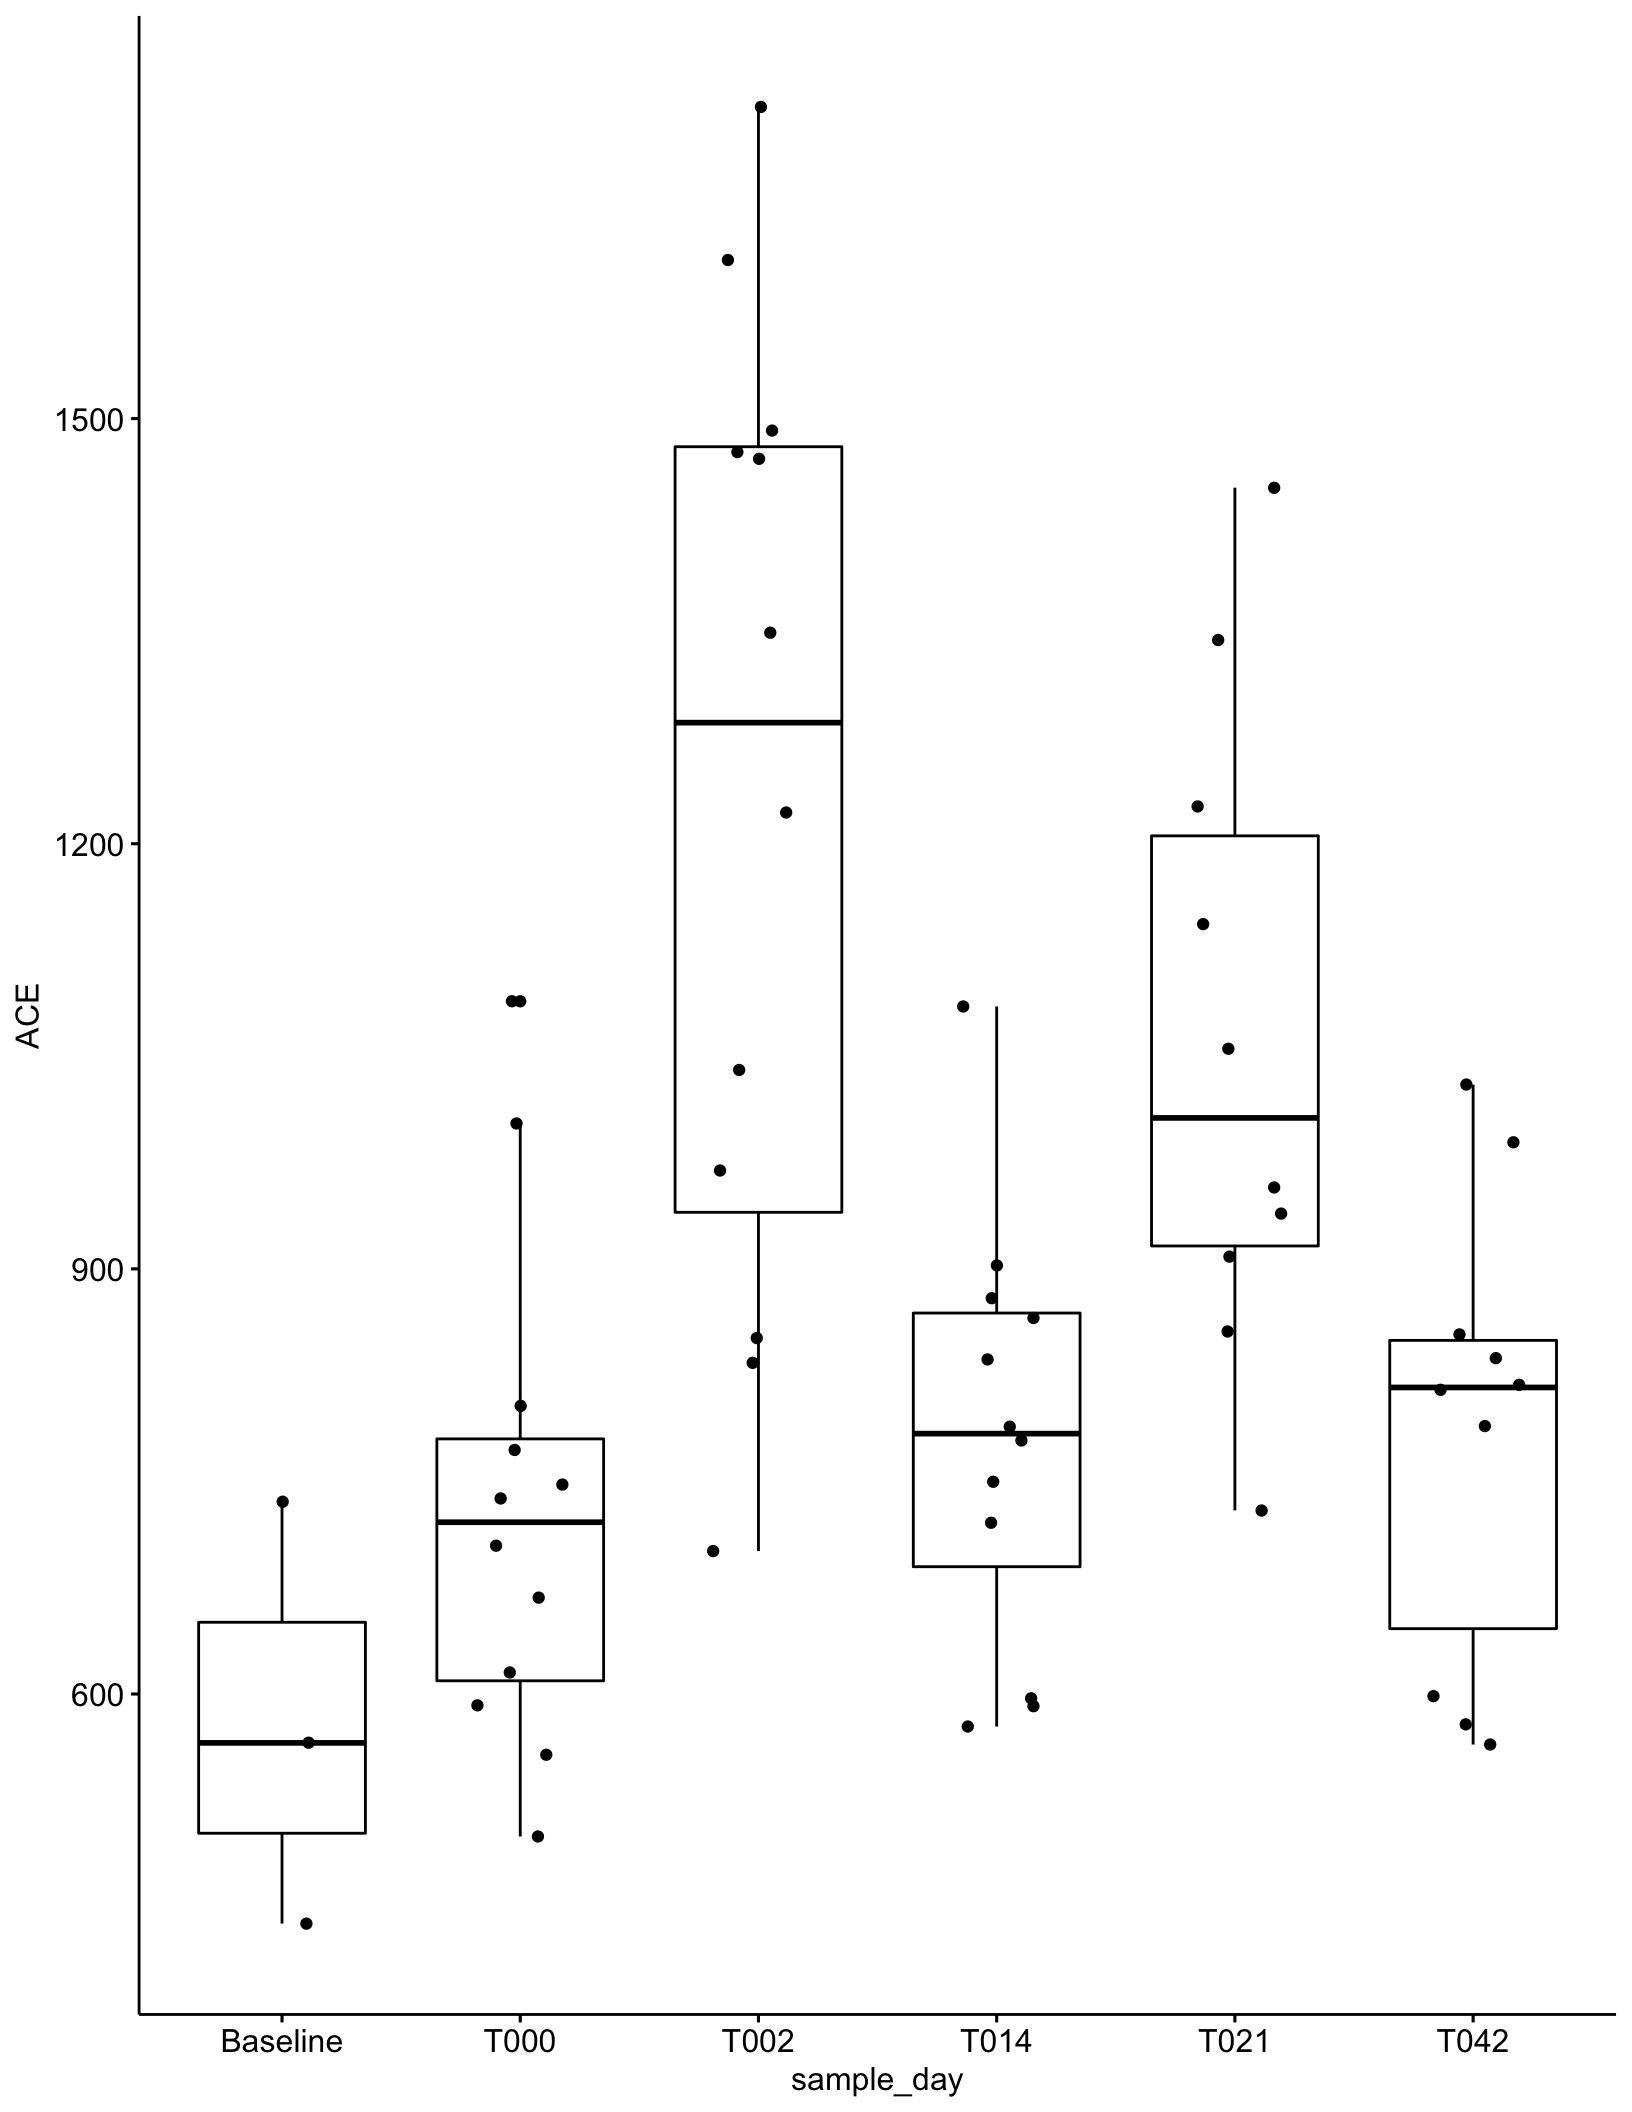
\includegraphics{cropprairiebetadiversity_files/figure-latex/unnamed-chunk-5-1.pdf}

\begin{Shaded}
\begin{Highlighting}[]
\NormalTok{d2rmintax10}
\end{Highlighting}
\end{Shaded}

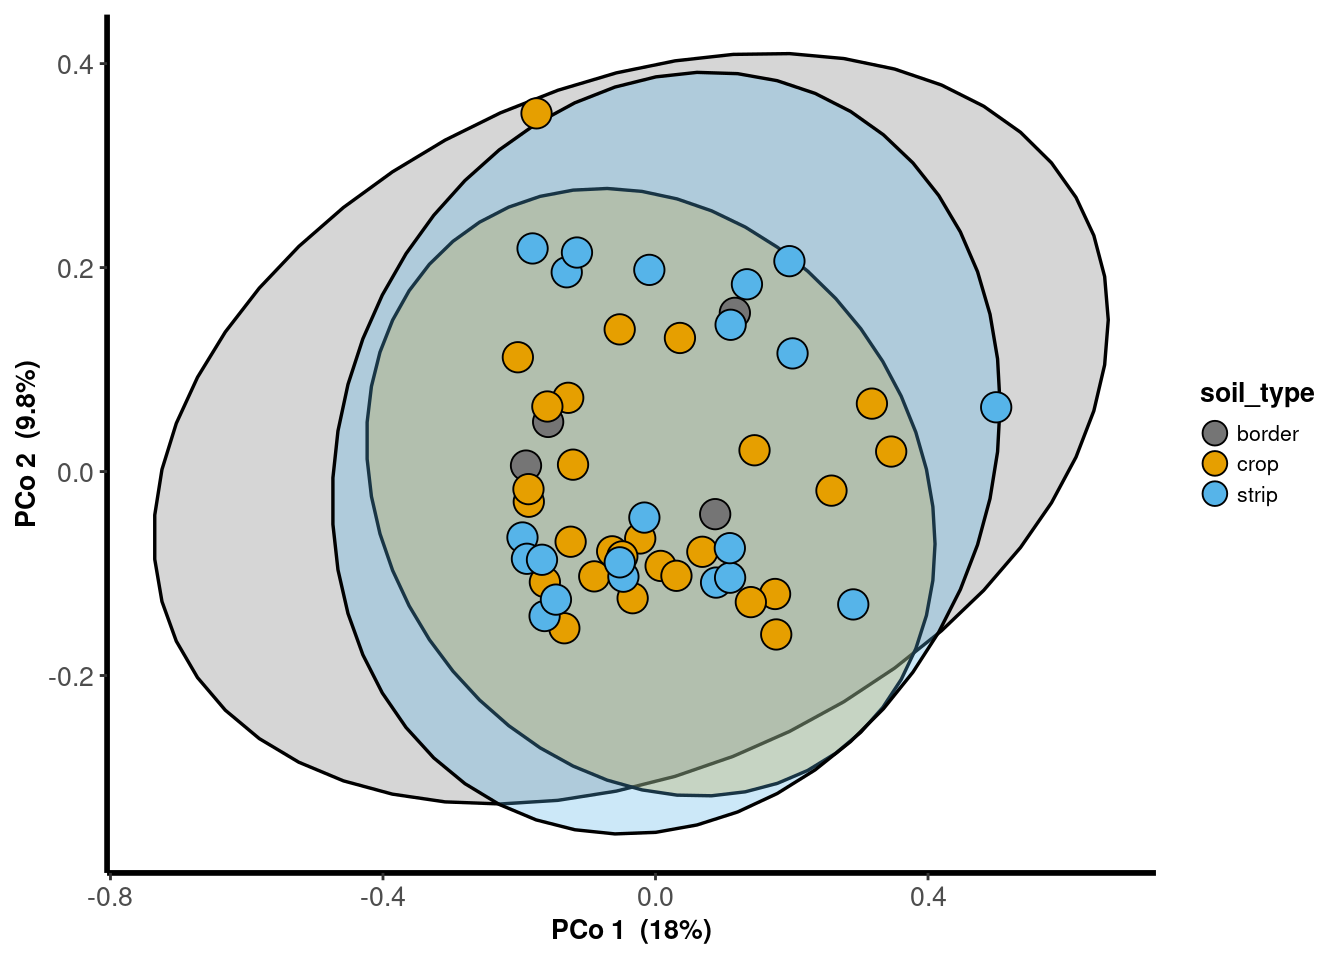
\includegraphics{cropprairiebetadiversity_files/figure-latex/unnamed-chunk-5-2.pdf}

\end{document}
